\chapter{Taking decisions} \label{cap:decidere}

\section{IF - AND, OR, NOT}

Now we want to give the Turtle the ability to take decisions but first let's make the scenario more interesting. 

So far we have depicted a sort of deterministic vision of computer programming. In our context this means giving the Turtle clear commands - do this, do that. Once the program is written the game is over. No matter the complexity, the drawing is frozen in the code. Thus, there is no place for randomness in the computer? Yes and no. A technical explanation for this answer would be too complex here. In a first approximation we can say that, no, a computer cannot produce true randomness but a sort of pseudo-randomness, thanks to appropriate mathematical tricks\footnote{Basically, in order to produce randomness one has to be able to generate random numbers, by means of so called random number generators. In reality, they generate periodic sequences, in the sense that after a certain number of numbers the same initial sequence is started again. The trick consists in using algorithms that produce extremely large periods so that one never reaches the end of the sequence by means of successive number extractions.}.

The Turtle understands the RANDOM command:

\begin{itemize}
\item X = RANDOM 100 ; gives back a random float\footnote{In computer science a float number is a number with decimal digits. For instance, 3.14 is a float number, 18 is an intenger number.} number (0 <= X < 100), that is equal or greater than 0 and smaller than 100
\item X = RANDOM “abcde” ; gives back a random letter among a, b, c, d, e
\item X = RANDOM [1, 2, 3] ; gives back a random element among 1, 2 and 3 - you can also mix different items, for instance RANDOM [1, “pippo”, 3.14]
\end{itemize}

In the aforementioned examples the random choices are memorized in the variable named X. Of course you can choose whatever name you prefer, or even use the instructions in some different way. For instance, try to play with the different use of the RANDOM command by means of the following code:

\vskip 1cm

\begin{scriptsize}
\begin{minipage}{0.50\textwidth}
\begin{itemize}[itemsep=-3pt,parsep=2pt, leftmargin=-0.0mm ]
\item[] HOME
\item[] CLEARSCREEN 
\item[] 
\item[] PENUP
\item[] FORWARD 300
\item[] 
\item[] REPEAT [
\item[] \hspace{8pt} LABEL RANDOM 100
\item[] \hspace{8pt} BACK 12
\item[] ]                      
\end{itemize}
\end{minipage}
\end{scriptsize}

\vskip 1cm

With this code the Turtle first goes next to the page top, then writes a column of ten successive RANDOM extraction by means of the LABEL instruction. Of course you can change whatever you like in this piece of code - it's always good to experiment.

Now, let's take a basic piece of code we are using several times, with variants:

\vskip 1cm

\begin{scriptsize}
\begin{minipage}{0.50\textwidth}
\begin{itemize}[itemsep=-3pt,parsep=2pt, leftmargin=-0.0mm ]
\item[] TO QUADRATO                 
\item[] \hspace{8pt} 	REPEAT 4 [ 
\item[] \hspace{8pt}\hspace{8pt}		FORWARD 100 
\item[] \hspace{8pt}\hspace{8pt}		RIGHT 90
\item[] \hspace{8pt}	]
\item[] END                            
\item[] 
\item[] QUADRATO
\end{itemize}
\end{minipage}
\end{scriptsize}

\vskip 1cm

This is the code to draw a square, as we have seen at the beginning of chapter \ref{cap:disegnare}. In chapter \ref{cap:ripetere} we investigated how to transform this code to get any kind of regular polygons. In a somewhat more complex variant, in chapter \ref{cap:marta}) we will explore more general cycles properties and in chapter \ref{cap:cerchio} we will discover the natural way of drawing a circle in the Turtle Geometry perspective, put in a practical didactic perspective: here just the code, to point out the similarity with the previous one.

\vskip 1cm

\begin{scriptsize}
\begin{minipage}{0.50\textwidth}
\begin{itemize}[itemsep=-3pt,parsep=2pt, leftmargin=-0.0mm ]
\item[] TO CERCHIO                 
\item[] \hspace{8pt} 	REPEAT 360 [ 
\item[] \hspace{8pt}\hspace{8pt}		FORWARD 1 
\item[] \hspace{8pt}\hspace{8pt}		RIGHT 1
\item[] \hspace{8pt}	]
\item[] END                            
\item[] 
\item[] CERCHIO
\end{itemize}
\end{minipage}
\end{scriptsize}

\vskip 1cm

Now, we have all the ingredients to give life to our Turtle. Let's inject a dose of randomness in the previous code. Within the repeating cycle, first we are going to tell the Turtle to move forward by a random amount between 1 and 2. In order to achieve this effect we write the instruction FORWARD RANDOM(1) + 1.  Here we are telling the Turtle to move forward by a quantity equal to RANDOM(1) +1. The command RANDOM(1)\footnote{At the beginning we showed a slightly different syntax: RANDOM 1 instead RANDOM(1). The first one is the standard LibreLogo version reported in the official LibreLogo Toolbar manual. The second one is an alternative version which is based on the underlying python code by means of which LibreLogo has been written. In the example we are discussing this version is preferable because it gives more clarity. Actually,  with the expression RANDOM 1 + 1 it is not clear if we are willing to sum 1  to the result of RANDOM 1 or if we want to call RANDOM 2. By using RANDOM(1) + 1 there is not such an ambiguity. } renders a random number between 0 and 1, thus, if we sum 1 to this, we obtain a random number which is comprised between 1 and 2. Second, we tell the Turtle to turn by a random amount, say between -45 and 45 degrees. We can achieve this result simlarly, by means of the instruction LEFT RANDOM(90) - 45, since with RANDOM(90) - 45 we get a random number between -45 and 45 degrees. 

Here we have the whole piece of code and its result:

\vskip 1cm

\begin{scriptsize}
\begin{minipage}{0.50\textwidth}
\begin{itemize}[itemsep=-3pt,parsep=2pt, leftmargin=-0.0mm ]
\item[] TO RANDOMMOVE
\item[] \hspace{8pt} 	REPEAT [ 
\item[] \hspace{8pt}\hspace{8pt}		FORWARD RANDOM(1) + 1 
\item[] \hspace{8pt}\hspace{8pt}		RIGHT RANDOM(90) - 45
\item[] \hspace{8pt}	]
\item[] END                            
\item[] 
\item[] RANDOMMOVE
\end{itemize}
\end{minipage}
\end{scriptsize}
\begin{minipage}{0.5\textwidth}
\begin{figure}[H]
   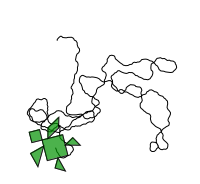
\includegraphics[width=3.0cm,trim=4 4 8 4,clip]{./images/decidere/decidere-1.png}
   \label{dec-2}
\end{figure}
\end{minipage} \hfill

\vskip 1cm

But be aware: if you are going to run repeatedly the same piece of code you will not be able to reproduce this drawing, or better: the probability of reproducing the same drawing is extremely low. So what? How can we be happy of producing unpredictable results by means of a machine conceived for making complex and accurate calculations? Well, actually, we are very glad because with this simple code we open a windows on the huge and crucial world of scientific simulation. Nowadays, in every scientific field the simulation is an essential investigation tool, the unique possible to face the overwhelming complexity of natural phenomena. Thus, what are we simulating here?





In questa versione proponiamo una descrizione estremamente sintetica. Giusto per completezza, perché il costrutto che si descrive è uno di quelli fondamentali in qualsiasi linguaggio di programmazione, oltre alle variabili, le ripetizioni e le procedure. Si tratta di disporre del modo per interrompere il flusso normale delle istruzioni, passando eventualmente a eseguire sezioni di codice diverse in dipendenza dello stato di certe variabili. L'istruzione che realizza questo in LibreLogo è \textbf{IF}, che per essere eseguita richiede la definizione di una condizione logica. Vediamo un esempio, riprendendo il codice per disegnare un cerchio, così come introdotto da Papert nel capitolo 2:



\vskip 1cm

\begin{scriptsize}
\begin{minipage}{0.50\textwidth}
\begin{itemize}[itemsep=-3pt,parsep=2pt, leftmargin=-0.0mm ]
\item[] TO CERCHIO                 
\item[] \hspace{8pt} 	REPEAT [ 
\item[] \hspace{8pt}\hspace{8pt}		FORWARD 1 
\item[] \hspace{8pt}\hspace{8pt}		RIGHT 1
\item[] \hspace{8pt}	]
\item[] END                            
\item[] 
\item[] CERCHIO                       
\end{itemize}
\end{minipage}
\end{scriptsize}

\vskip 1cm

Se facciamo girare questo codice la Tartaruga disegna un cerchio ma non si
ferma mai, ripassandolo infinite volte. Naturalmente noi possiamo fermarla con
il tasto 
\includegraphics[height=1em]{./images/ripetere/StopLO.png}, ma è possibile insegnarle a fermarsi da sola. Ecco come:

\vskip 1cm

\begin{scriptsize}
\begin{minipage}{0.50\textwidth}
\begin{itemize}[itemsep=-3pt,parsep=2pt, leftmargin=-0.0mm ]
\item[] TO CERCHIO                 
\item[] \hspace{8pt} 	REPEAT [ 
\item[] \hspace{8pt}\hspace{8pt}		FORWARD 1 
\item[] \hspace{8pt}\hspace{8pt}		RIGHT 1
\item[]	\hspace{8pt}\hspace{8pt}		\textbf{IF REPCOUNT = 90 [ STOP ]}
\item[] \hspace{8pt}	]
\item[] END                            
\item[] 
\item[] CERCHIO                       
\end{itemize}
\end{minipage}
\end{scriptsize}

\vskip 1cm

Come si vede, abbiamo aggiunto una sola istruzione, \textbf{IF REPCOUNT = 90 [ STOP ]}, che equivale a dire alla Tartaruga: se il contatore dei cicli ha raggiunto il valore di 90 allora fermati. Siccome ad ogni ciclo ruota di 1 grado, in questo modo ne interrompiamo il disegno quando in totale avrà ruotato di 90 gradi, ovvero quando avrà disegnato un quarto di cerchio. Provare e variare per vedere...
La condizione in questo esempio è espressa da REPCOUNT = 90. Si  possono usare anche gli operatori “minore di”, <, e “maggiore di”, >, e le condizioni si possono combinare insieme con gli operatori logici AND, OR e NOT. L'AND posto fra due condizioni crea una condizione globale vera se sono ambedue vere. L'OR posto fra due condizioni crea una condizione globale vera se sono ambedue vere oppure anche una sola delle due. Il NOT posto prima di una condizione ne inverte l'esito: la rende falsa se è vera e viceversa. Inoltre si può costruire l'istruzione in maniera che se questa è vera esegue una prima sezione di codice, mentre se è falsa ne  esegue un'altra. In questa versione del manuale ci limitiamo a riportare giusto un esempio riassuntivo:

\vskip 1cm

\begin{scriptsize}
\begin{minipage}{0.80\textwidth}
\begin{itemize}[itemsep=-3pt,parsep=2pt, leftmargin=-0.0mm ]
\item[]	\textbf{IF A $<$ 10 AND NOT A = 5 [ PRINT "Vero!" ] [ PRINT "Falso!" ]}                      
\end{itemize}
\end{minipage}
\end{scriptsize}

\vskip 1cm

Tradotto in parole: se la variabile A è minore di 10 e allo stesso tempo (AND), è diversa da 5 (NOT), allora esegui PRINT “Vero!”, altrimenti esegui PRINT “Falso!”.







